\documentclass[draft,a4paper]{ctexart}
\usepackage{mathtools,amsfonts}
\usepackage{hyperref}
\graphicspath{{figures/}}
\title{不平衡数据分类及其在点击率预估上的应用}
\author{张航}
\begin{document}
\maketitle

不平衡数据(imbalanced data set, IDS)是指不同类别的样本量差异很大的数据集.
比如对二分类问题,IDS中多数类和少数类样本的比例可能高达\(100:1\),
\(1000:1\),甚至\(10000:1\).
IDS出现在多种互联网应用场景中,如广告的点击率预测(点击率通常很小),
电子商务领域的商品推荐(推荐的商品被购买的比例很低),
交易欺诈检测(真正欺诈的人占少数),网络攻击识别等等。
本文先对一般的分类问题讨论IDS带来的问题及解决方法,再针对
点击率(click-through rate, CTR)预估给出一些具体的做法和实际例子.

\section{不平衡性带来的问题}
\subsection{分类面偏移}
传统的分类方法, 大都建立在训练样本数量均衡的前提下,
当用于解决不平衡分类问题时,
它们往往在多数类的分类精度较高而在少数类的分类精度很低.
\begin{figure}[tbp]
  \centering
  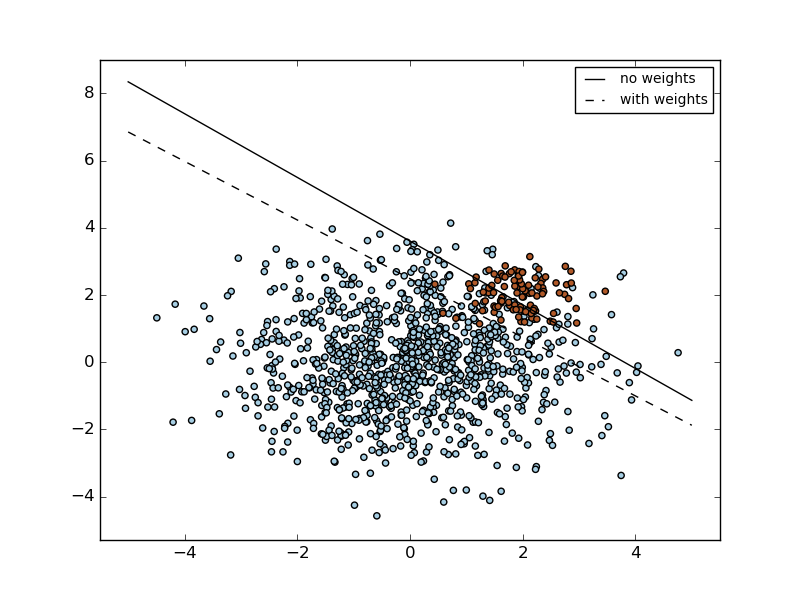
\includegraphics[width=.8\textwidth]{svm_unbalanced}
  \caption{IDS引起SVM决策面偏移: 实线是直接训练出的分类面,
  虚线是增大少数类权重后的分类面}
  \label{fig:svm_sep}
\end{figure}
Japkowicz等\cite{japkowicz2002class}通过实验发现
在大规模训练样本上不平衡性对分类器性能的不良影响较小,
同时减少概念复杂度(concept complexity), 即特征稀疏或者
取值范围较小, 也能改善分类器表现.

\subsection{评测指标问题}
传统的分类方法一般以准确率作为评测指标,
但是IDS上分类器倾向于降低稀有类的分类效果,
这样准确率就不能很好反应稀有类对分类性能评测的影响.
例如,假设有一个训练样本数量为 1∶99的两类问题 ,即使分类器将所
有样本分到大类 ,它仍可以得到 99\%的训练准确率.

\section{解决策略}
\subsection{重采样(re-sampling)}
重采样方法通过增加小类样本数的上采样(up-sampling)
和减少大类样本数的下采样(down-sampling)使不平衡的样本分布变得
比较平衡, 从而提高分类器对小类的识别率.
\subsubsection{上采样(up-sampling)}
当小类样本的绝对数量较小时需要上采样.
最原始的上采样方法是复制小类样本,
但是这样容易导致过拟合.
Chawla等\cite{chawla2002smote}提出的Synthetic Minority Oversampling
Technique(SMOTE)是一种简单有效的上采样方法,
该方法首先为每个稀有类样本随机选出几个邻近样本,
并且在该样本与这些邻近的样本的连线上随机取点,
生成无重复的新的稀有类样本, 如\autoref{fig:smote}所示.
\begin{figure}[htpb]
  \centering
  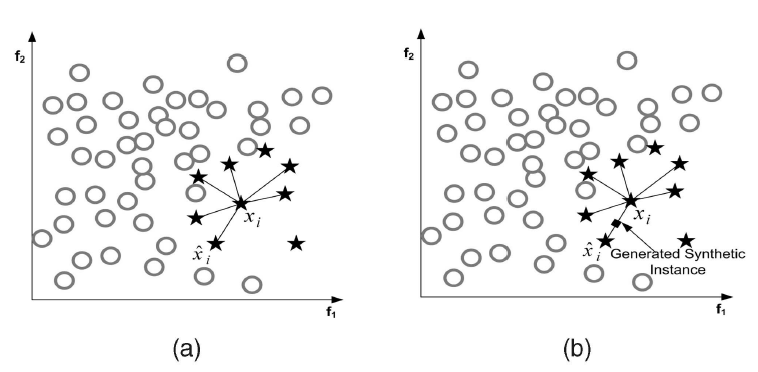
\includegraphics[width=.8\textwidth]{smote}
  \caption{SMOTE算法:(a)对点\(x_i\)找到同类近邻\(\hat{x}_i\);
  (b)在\(x_i, \hat{x}_i\)的连线上随机生成新点}
  \label{fig:smote}
\end{figure}
\subsubsection{下采样(down-sampling)}

\subsection{训练集划分}

\subsection{代价敏感学习(cost sensitive learning)}

\subsection{评测指标}

\section{CTR应用}
\subsection{CTR特点}
\subsection{下采样}
\subsection{经验结果}

\bibliographystyle{alpha}
\bibliography{ref}
\end{document}
